\section{Mapeo de características}

\subsection{Introducción}

Utilizando el mismo dataset de Bag of Words (BOW) del ejercicio anterior debemos construir un modelo de mapeo de características auto-organizado que clasifique automáticamente los 
documentos en un arreglo de dos dimensiones. Este problema será resuelto utilizando Kohonen.

Kohonen:
\begin{itemize}
	\item Propone un orden topológico y un modelo competitivo
	\item Función de transferencia 
				\begin{align*}
					O_{i}=f(\varepsilon, W_{i}) donde W_{i}=(w_{i1}, ..., w_{in}) \in \mathbb{R}_{n}
				\end{align*}
	
	\item PRINCIPIO DE ADAPTACIÓN: Consiste en detectar la unidad cuyos parámetros sean más parecidos a la entrada $\varepsilon$.
		\begin{itemize}
			\item Establece un orden topológico y solo se cambian los parámetros de la unidad seleccionada y los de sus vecinas.
			\item El cambio es en dirección de incrementar la sililaridad entre $W_{i}$ y $\varepsilon$.
			\item La magnitud del cambio debe garantizar estabilidad asintótica.
		\end{itemize}
		Estas tres cosas hacen que la función de densidad de probabilidades de $W_{i}$ tienda a aproximar la densidad $P(\varepsilon)$.
	\item MAPAS DE KOHONEN: Es una propuesta de implementación la cual define:
		\begin{itemize}
			\item Que la unidad seleccionada en tiempo $t$ será $c$ tal que:
				\begin{align*}
					||\varepsilon(t) - W_{c}(t)|| = min\{\varepsilon(t) - W_{i}(t)\}
				\end{align*}
			
			\item Se establece una topología de entrada a partir de establecer funciones de vecindad, esto fuerza a que los pesos no crezcan de una forma desmedida respecto de los 
			pesos de las unidades vecinas. Esto hace que los entornos sean amplios al principio pero pequeños al final, hasta limitarse solo a la unidad seleccionada.
				
			\item REGLA DE KOHONEN: Actualización de los $W_{i}$.
					\begin{align*}
					 W_{i}(t+1) &=  \begin{cases}
										W_{i}(t) + \alpha(t) [ \varepsilon(t) - W_{i}(t) ] & i \in N_{c} \\
										W_{i}(t)                                           & i \not \in N_{c}  
									\end{cases} \\
					\end{align*}
			\item $\eta(t)$ es el coeficiente de aprendizaje dinámico, decreciente en el tiempo.
				\begin{align*}
					\Delta W_{ij} = \alpha(t) [ \varepsilon(t) - W_{i}(t) ]
				\end{align*}
				\begin{align*}
					\alpha(t) = \eta \Lambda(i,c)
				\end{align*}
				\begin{align*}
					\Lambda(i,c) = \begin{cases}
										1 & i = c \\
										decrece a mayor distancia entre i y c 
									\end{cases} \\
				\end{align*}
		\end{itemize}
	\item TEOREMA DE KOHONEN: Con probabilidad 1 los $W_{i}$ se ordenan de forma ascendientes o descendientes cuando $t \to
		\infty$ si $\alpha(t) \to 0$ con suficiente lentitud.
\end{itemize}

\subsection{Modelo}
Al igual que en el ejercicio anterior, el conjunto de datos contiene 900 documentos con 856 descripciones de texto 
correspondientes a compañías Brasileñas clasificadas en nueve categorías distintas.

En primer lugar sabemos que la red a entrenar tendrá un aprendizaje no supervisado, ya que no sabemos el resultado al que
queremos llegar.

Para diseñar la estructura de la red debemos saber cuantas clases existen en el dataset, como dijimos anteriomente son nueve.

Sabemos que unidades de entradas cercanas deben activar unidades de salidas cercanas.

Definimos:
\begin{align*}
	n, M, M_{1}, M_{2} \in \mathbb{N} \\
	M = M_{1} . M_{2} \\
	X \in \mathbb{R}_{n} \\
	Y \in \mathbb{R}_{M} \\
	W \in \mathbb{R}_{n.M} \\
\end{align*}

donde:

$Y$ es el vector de entrada.

$W$ es la matriz de pesos asociado a cada par de neuronas. 

$X$ es el vector de salida de nuestra red, cuyos índice $i$ indicará el número de unidad. Dicho índice contiene una matriz con
 los pesos $W_{i}$ asociado a cada neurona $j$.\\

Para calcular la activación de una capa Kohonen ve cuánto estímulo recibe una neurona de la capa anterior y ve cuál se activa.
Para saber cula se activa debemos establecer un criterio de activación. Elegimos a la unidad ganadora como el $j$ que más se 
parece a mi vector de entrada y con esto sabemos que es la neurona que se encuentra a menor distancia. 

En nuestro caso utilizamos la distancia euclidiana:

\begin{align*}
		j* = argmin_{j}||Y^{T} \bullet W_{\bullet j}(t)||_{2}
\end{align*}

De esta forma calculamos la distancia entre $Y$ y cada columna de $W$ y posteriomente nos quedamos con la neurona $j$ 
cuya distancia minimiza la función. En la figura 2, mostramos cómo se realiza dicha comparación teniendo en cuenta las dimensiones.

\newpage

\begin{figure}[ht!]
	\centering
	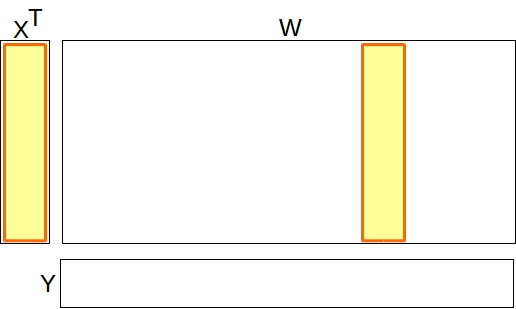
\includegraphics[width=0.7\linewidth]{img/parte2-comparacion.jpg}
	\caption{Comparación}
\end{figure}

El vector X tiene dimensión $1 x M$ con $M = M_{1} . M_{2}$. Esto indica que el vector $M$ esta formado por $M_{2}$ vectores $M_{1}$.
EXPLICAR ESTO!!!!!!!

Con esto logramos que una salida se apodere de un sector de la entrada y en consecuencia puede llegar a suceder que en nuestra red
no haya un orden topológico. Por lo tanto, una vez elegida la neurona ganadora debemos implementar una topología de entrada.
La topología que utilizamos se muestra en la siguiente figura.

\begin{figure}[ht!]
	\centering
	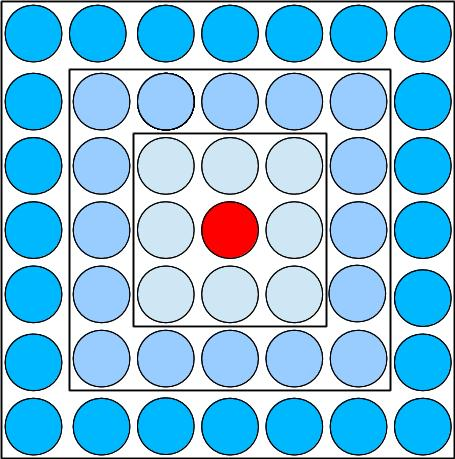
\includegraphics[width=0.3\linewidth]{img/parte2-vecindario.jpg}
	\caption{Función de vecindario.}
\end{figure}

Este tipo de topología fuerza a que los pesos no crezcan en forma desmedida con respecto a las neuronas vecinas. 
Dichos pesos los 
actualizamos mediante la Regla de Kohonen:

\begin{align*}
	W_{i}(t+1) &=  \begin{cases}
						W_{i}(t) + \alpha(t) [ \varepsilon(t) - W_{i}(t) ] & i \in N_{c} \\
						W_{i}(t)                                           & i \not \in N_{c}  
					\end{cases} \\
\end{align*}


Para que un modelo sea auto-organizado debemos elegir el sigma $\sigma$ y  el eta $\eta$ adecuados. El sigma será 
utilizado como parámetro de la Gauseana y medirá la dispersión, cuantas neuronas vecinas a la neurona activada modificarán 
sus pesos. Por otro lado, el $\eta$ será el coeficiente de aprendizaje de nuestra red.







\begin{figure}[ht!]
	\centering
	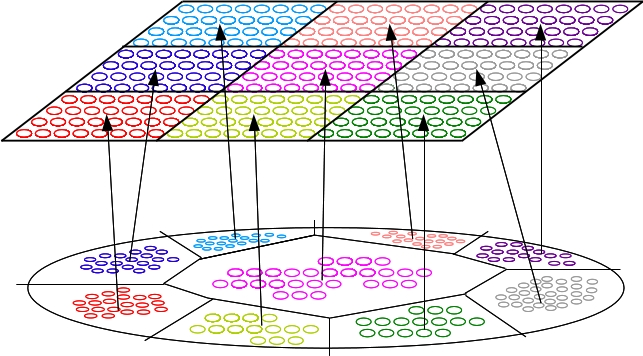
\includegraphics[width=0.8\linewidth]{img/parte2-kohonen9clases.jpg}
	\caption{Clasificación con Kohonen}
\end{figure}

